\documentclass{article}

\usepackage{graphicx}
\usepackage{tikz}
\usepackage{tikzsymbols}
\usetikzlibrary{calc,patterns,shapes.geometric}
\pagestyle{empty}
\usepackage[margin=0pt]{geometry}
\geometry{papersize={14in,12in}}

\def\centerarc[#1](#2)(#3:#4:#5){\draw[#1] ($(#2)+({#5*cos(#3)},{#5*sin(#3)})$) arc (#3:#4:#5);}

\begin{document}
	\begin{figure}
		\centering
		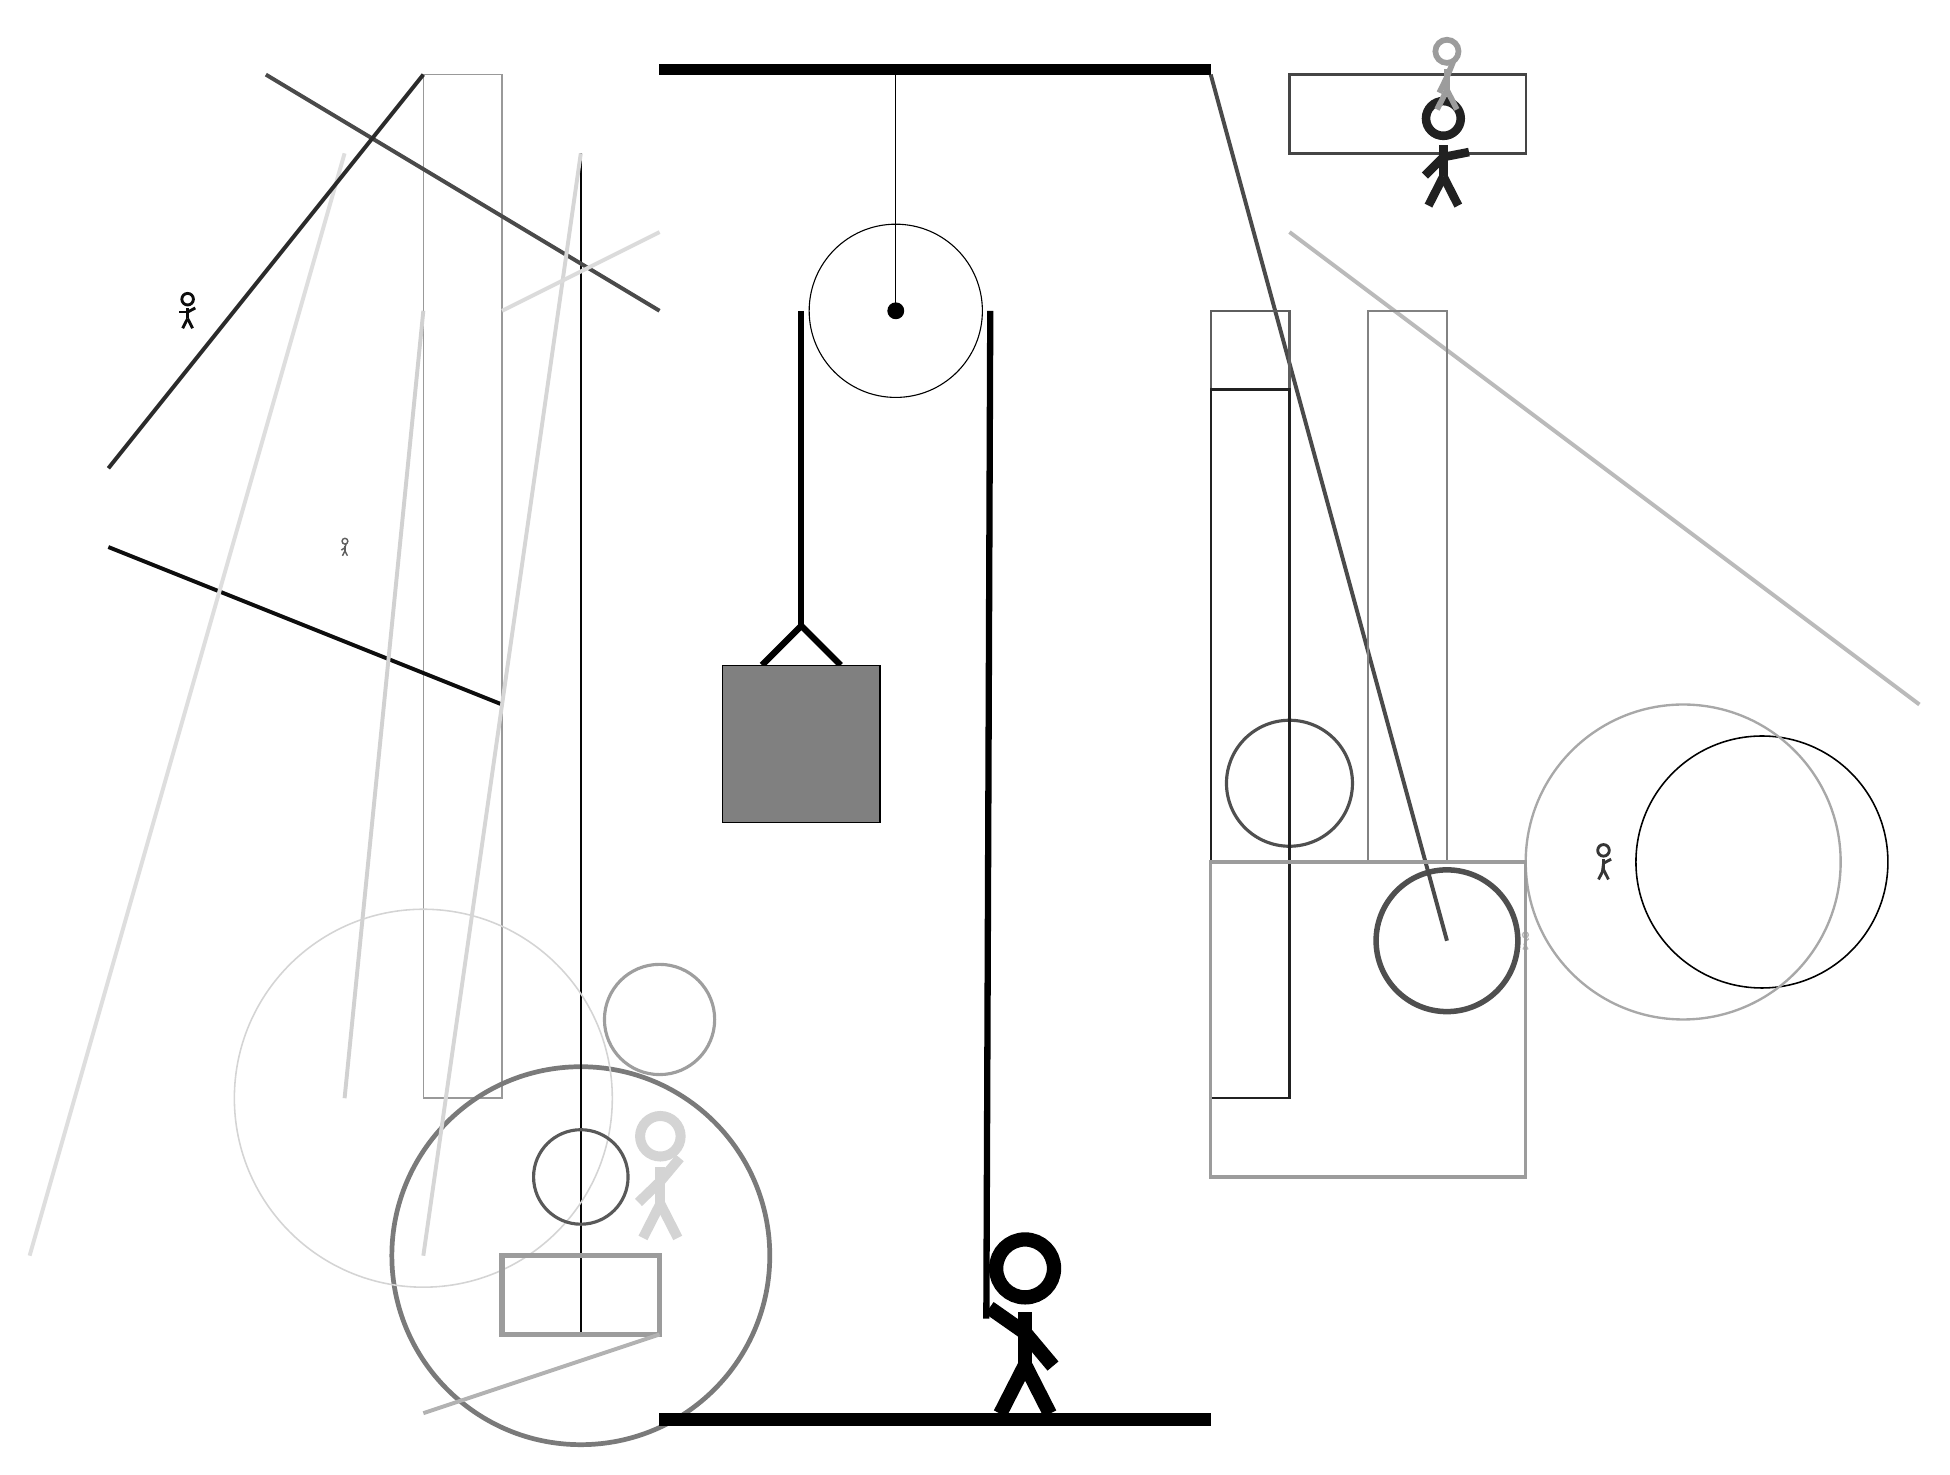
\begin{tikzpicture}
			%%%%% START %%%%%
			
			\draw[fill=black] (-2, 14) rectangle (5, 14.125);
			
			\draw (1, 11) circle (1.1);
			\draw[fill=black] (1, 11) circle (0.1);
			\draw (1, 14) -- (1, 11);
			
			\draw[line width=0.8mm] (-0.7, 6.5) -- (-0.2, 7.0) -- (0.3, 6.5);
			\draw[fill=black!50] (-1.2, 6.5) rectangle (0.8, 4.5);
			
			\draw[line width=0.8mm] (-0.2, 11) -- (-0.2, 7.0);
			\centerarc[line width=0.8mm](1, 11)(0:180:1.2000000000000002);
			\draw[line width=0.8mm](2.2, 11) -- (2.15, -1.8);
			
			\node at (2.6, -1.9) {\Strichmaxerl[10][-35][-50]};
			
			\draw [line width=0.7mm, color=black!69](8, 3) circle (0.9);
			
			\draw[line width=0.2mm, color=black!40] (-4, 1) rectangle (-5, 14);
			\draw[line width=0.3mm, color=black!73] (6, 13) rectangle (9, 14);
			\draw[line width=0.5mm, color=black!95](-4, 6) -- (-9, 8);
			
			\draw [line width=0.2mm, color=black!100](12, 4) circle (1.6);
			\draw [line width=0.3mm, color=black!34](11, 4) circle (2.0);
			
			\draw [line width=0.6mm, color=black!52](-3, -1) circle (2.4);
			\draw[line width=0.2mm, color=black!98] (-3, -2) rectangle (-3, 13);
			\node[line width=0.2mm, color=black!87] at (8, 13) {\Strichmaxerl[6][45][11]};
			
			\draw[line width=0.5mm, color=black!18](-5, 11) -- (-6, 1);
			\node[line width=0.4mm, color=black!95] at (-8, 11) {\Strichmaxerl[2][0][28]};
			\draw [line width=0.2mm, color=black!17](-5, 1) circle (2.4);
			\node[line width=0.2mm, color=black!27] at (9, 3) {\Strichmaxerl[1][68][39]};
			\draw[line width=0.7mm, color=black!39] (-4, -2) rectangle (-2, -1);
			\draw[line width=0.5mm, color=black!71](-7, 14) -- (-2, 11);
			\draw[line width=0.5mm, color=black!71](5, 14) -- (8, 3);
			\draw [line width=0.4mm, color=black!69](6, 5) circle (0.8);
			\draw[line width=0.3mm, color=black!63] (6, 11) rectangle (5, 10);
			\node[line width=0.7mm, color=black!17] at (-2, 0) {\Strichmaxerl[7][44][50]};
			\draw[line width=0.5mm, color=black!27](6, 12) -- (14, 6);
			\draw [line width=0.4mm, color=black!38](-2, 2) circle (0.7);
			
			\node[line width=0.4mm, color=black!39] at (8, 14) {\Strichmaxerl[4][64][68]};
			\draw[line width=0.5mm, color=black!16](-5, -1) -- (-3, 13);
			\node[line width=0.6mm, color=black!63] at (-6, 8) {\Strichmaxerl[1][34][73]};
			\draw [line width=0.4mm, color=black!65](-3, 0) circle (0.6);
			
			\draw[line width=0.5mm, color=black!13](-6, 13) -- (-10, -1);
			\draw[line width=0.5mm, color=black!14](-4, 11) -- (-2, 12);
			\draw[line width=0.5mm, color=black!30](-2, -2) -- (-5, -3);
			\draw[line width=0.2mm, color=black!49] (7, 11) rectangle (8, 4);
			\draw[line width=0.5mm, color=black!83](-5, 14) -- (-9, 9);
			\draw[line width=0.3mm, color=black!87] (5, 10) rectangle (6, 1);
			\draw[line width=0.4mm, color=black!39] (5, 0) rectangle (9, 4);
			\node[line width=0.4mm, color=black!79] at (10, 4) {\Strichmaxerl[2][83][28]};
			
			\draw[fill=black] (-2, -3) rectangle (5, -3.15);
			
			%%%%% END %%%%%
		\end{tikzpicture}
	\end{figure}	
\end{document}